\documentclass[serif, pdf]{beamer}

%   Theme
\usetheme{Warsaw}

%   Packages
\usepackage{xcolor}
\usepackage{tikz}
\usepackage{multimedia}
\usepackage{lmodern}
\usepackage{scrextend}
\usepackage{subcaption}
%\usepackage{media9}
%\usepackage{movie15}

%   To keep the spacing of text in tables
\usepackage{makecell}
%   Parameter for the spacing
\setcellgapes{4pt}

\usepackage{caption}
%   Redefines the caption setup of the Figures environment in the beamer class
\captionsetup[figure]{labelformat=empty}
\setbeamerfont{caption}{size=\scriptsize}

%   Colour theme
\usecolortheme{beaver}

%   Metadata
\title[SAIMechE]{Project Title}
\date{22 November 2019}
\author[Naud\'e Conradie]{Naud\'e Conradie\\{\small Supervisor: Dr MP Venter}}
\institute[]{Department of Mechanical and Mechatronic Engineering, Stellenbosch University}

%   Colour definitions
\definecolor{colour1}{RGB}{96, 34, 59}
\definecolor{colour2}{RGB}{140, 151, 154}
\setbeamercolor{structure}{fg=colour1,bg=colour2}
\setbeamercolor{title}{fg=white,bg=colour2}
\setbeamercolor{author in head/foot}{fg=colour1}

%   Beamer template settings
\setbeamertemplate{itemize item}{\color{black}$\bullet$}
\setbeamertemplate{itemize subitem}{\color{black}$-$}
\setbeamertemplate{caption}{\raggedright\insertcaption\par}

%   Footer settings
\expandafter\def\expandafter\insertshorttitle\expandafter{%
  \insertshorttitle\hfill%
  \hspace{30mm}\insertframenumber\,/\,\inserttotalframenumber}

\beamertemplatenavigationsymbolsempty

\begin{document}

%   Title Slide-------------------------------------------------%

\begin{frame}
  \begin{center}
    \vspace{0.1cm}
    \includegraphics[scale=0.25]{USlogo.pdf}
  \end{center}
  \titlepage
\end{frame}

%   Overview----------------------------------------------------%

\changefontsizes{13pt}
\begin{frame}
    \frametitle{Overview}
    \begin{itemize}
        \item<1-> Project scope
        \item<2-> Background
        \item<3-> Results
        \item<4-> Objectives
    \end{itemize}
\end{frame}

%   Project Scope-----------------------------------------%

\begin{frame}
    \frametitle{Project Scope}
    \begin{itemize}
        \item<1-> Automate design of shape-changing soft robots
        \changefontsizes{11pt}
        \begin{itemize}
            \item<2-> Change internal pressure
        \end{itemize}
        \item<3-> Non-linear FEM
        \changefontsizes{11pt}
        \begin{itemize}
            \item<4-> Restricted to two dimensions
        \end{itemize}
    \end{itemize}
\end{frame}

%   Project Scope-----------------------------------------%

\begin{frame}
    \frametitle{Project Scope (cont.)}
    \begin{itemize}
        \item<1-> Computationally efficient
        \changefontsizes{11pt}
        \begin{itemize}
            \item<2-> Use recursive grammatical encodings
            \item<3-> L-systems for cellular level
            \item<4-> CPPNs for organism level
        \end{itemize}
        \item<5-> Evolve a population to obtain best model
    \end{itemize}
\end{frame}

%   Background----------------------------------------------------%

\begin{frame}
    \frametitle{Background}
    \begin{minipage}{0.7\textwidth}
        \begin{itemize}
            \item<1-> Soft robotic bodies are computationally expensive
            \item<2-> Lindenmayer systems
            \begin{itemize}
                \item<3-> Recursive grammatical encodings
                \item<4-> Built from set of rules, axioms, variables and constants
                \item<5-> CPPNs for organism level
            \end{itemize}
            \item<3-> N Cheney et al. - Unshackling evolution
            \item<3-> J Hiller \& H Lipson - Evolving amorphous robots
            \item<3-> J Rieffel et al. - Growing and evolving soft robots
            \item<4-> M Aiguier et al. - Emergent properties in reactive systems
           
            \item<5-> N Kim - Introduction to nonlinear finite element analysis
        \end{itemize}
    \end{minipage}
    \begin{minipage}{0.25\textwidth}
        \begin{figure}
            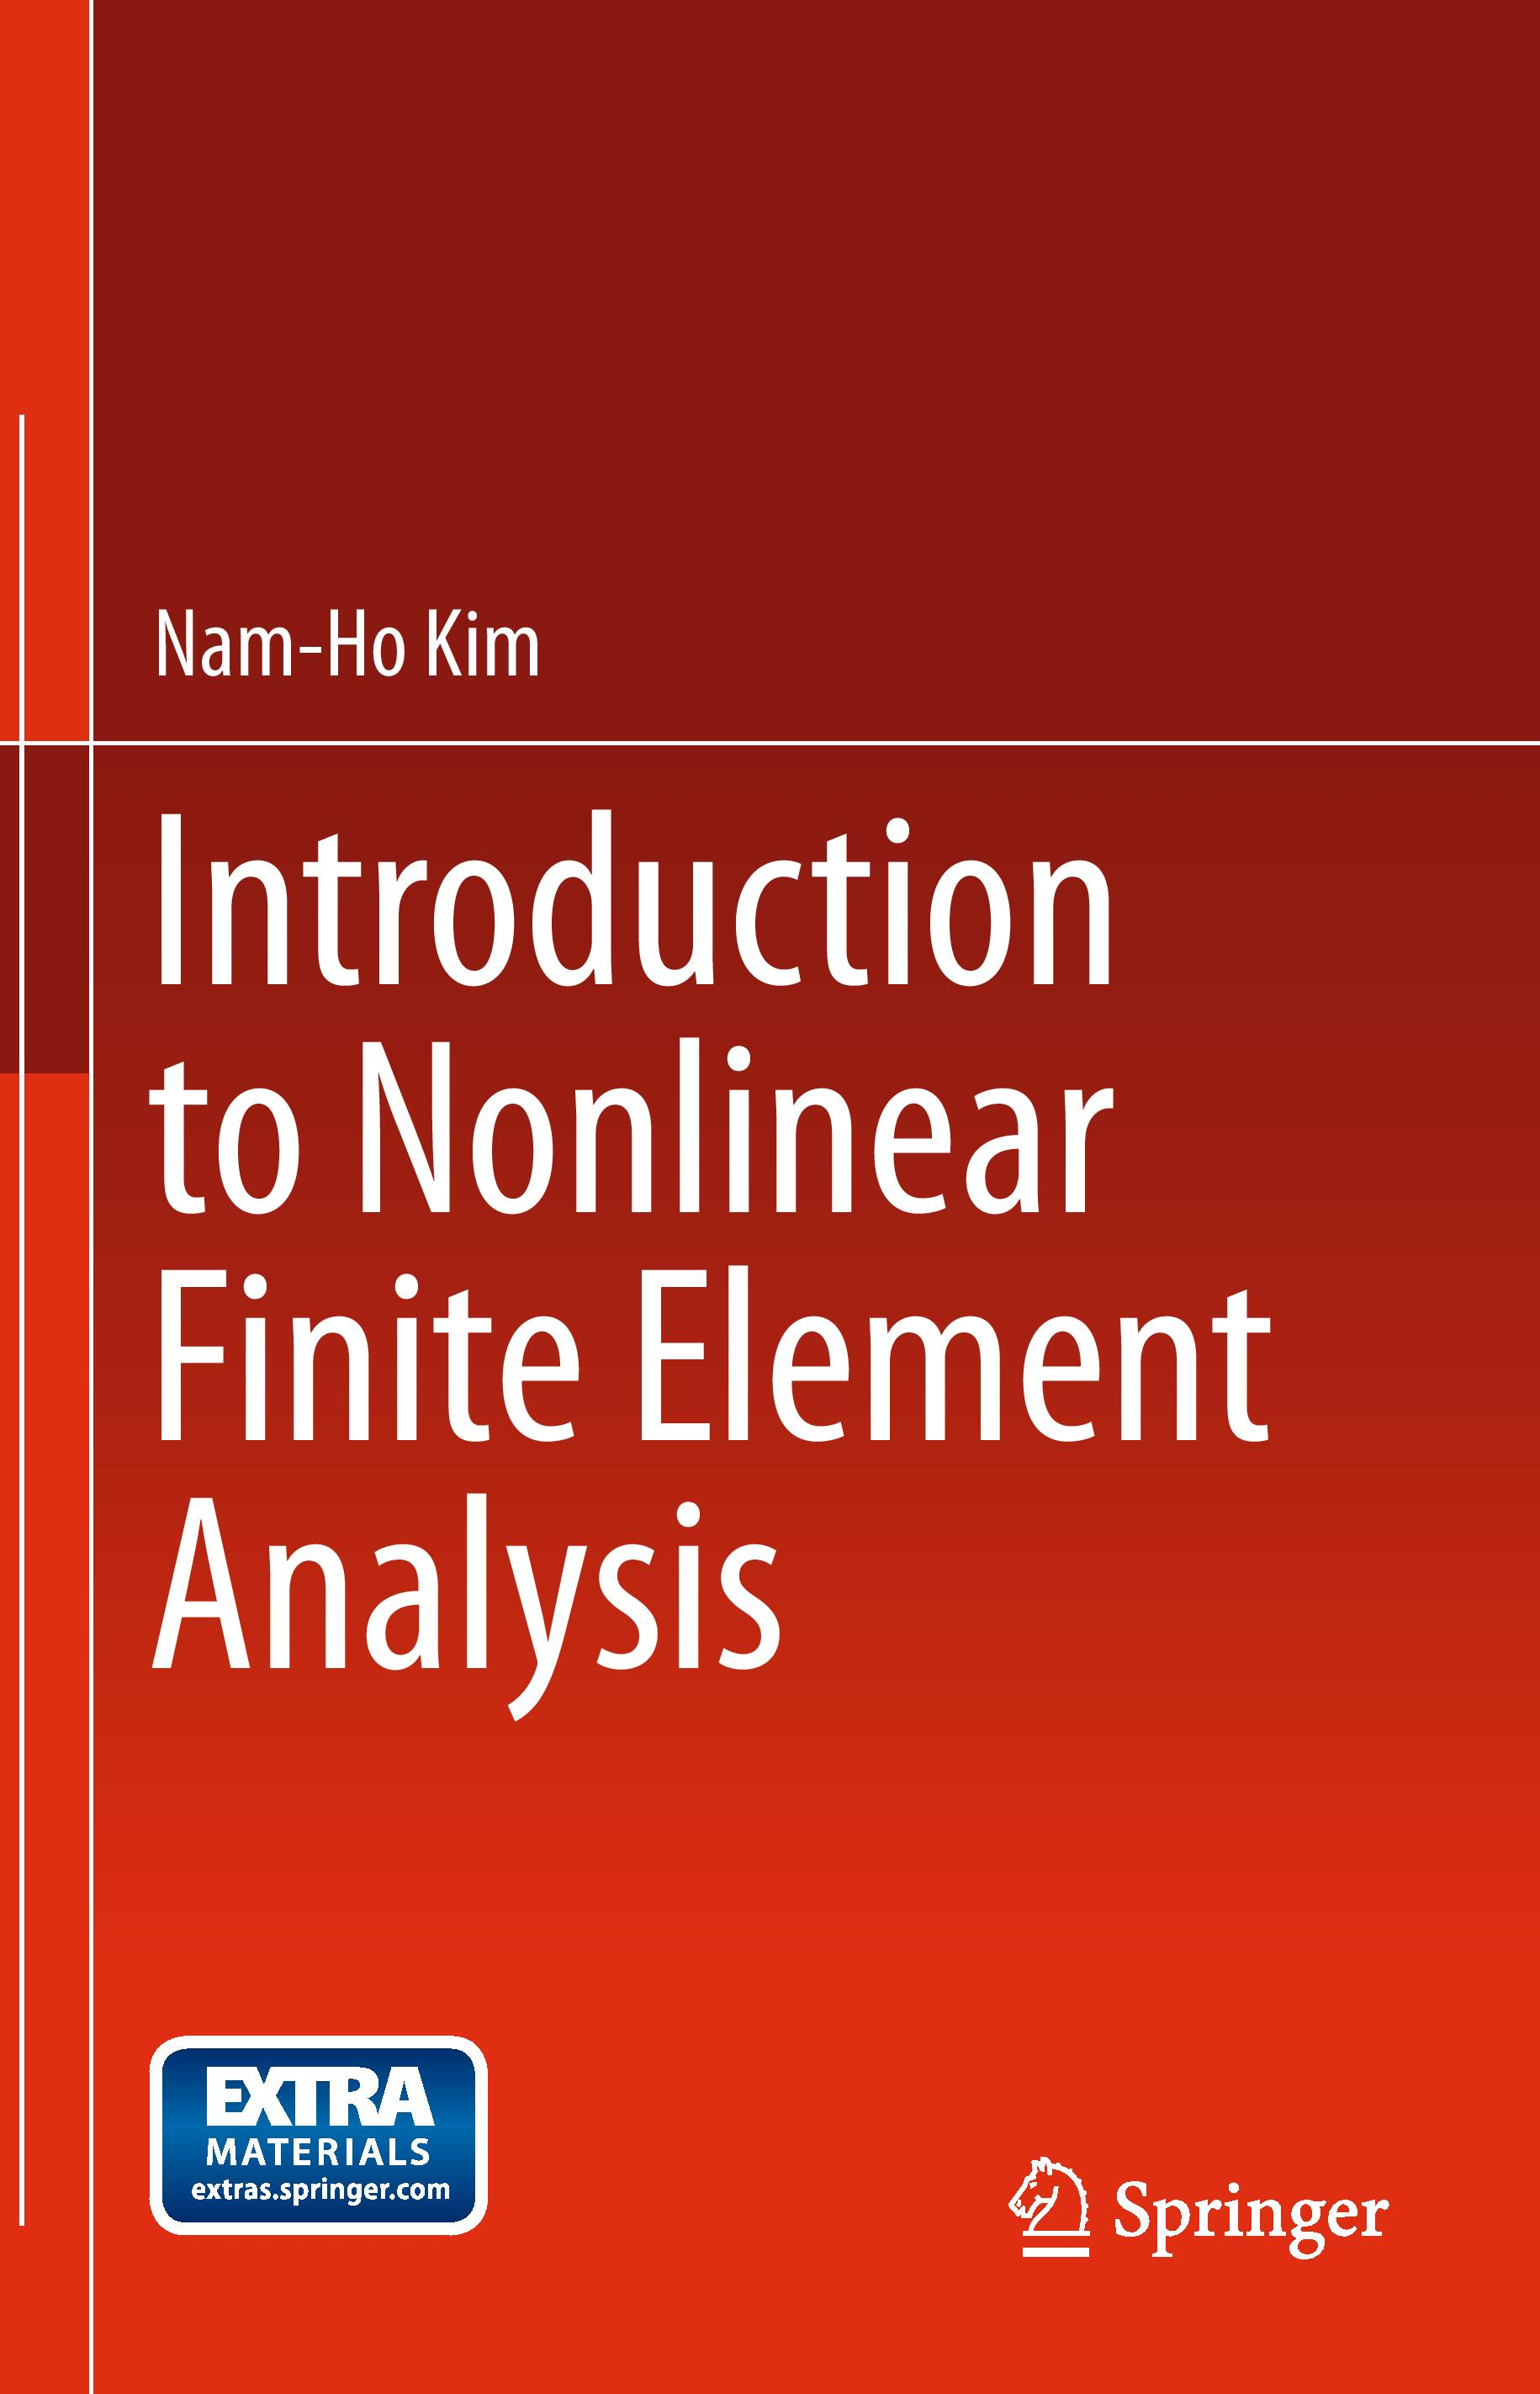
\includegraphics[height = 5cm]{Textbook_Cover_Page.jpg}<5->
        \end{figure}
    \end{minipage}
\end{frame}

%   Current Objectives------------------------------------------%

\begin{frame}
    \frametitle{Current Objectives}
    \begin{itemize}
        \item<1-> 10x10 empty grid of 2D elements
        \item<2-> Applying external pressure
        \item<3-> Linear vs hyperelastic material
        \changefontsizes{11pt}
        \begin{itemize}
            \item<4-> Material status completely describable with given total strain
            \item<5-> Mold-star 15
        \end{itemize}
    \end{itemize}
    \begin{subfigure}{.5\textwidth}
        \centering
        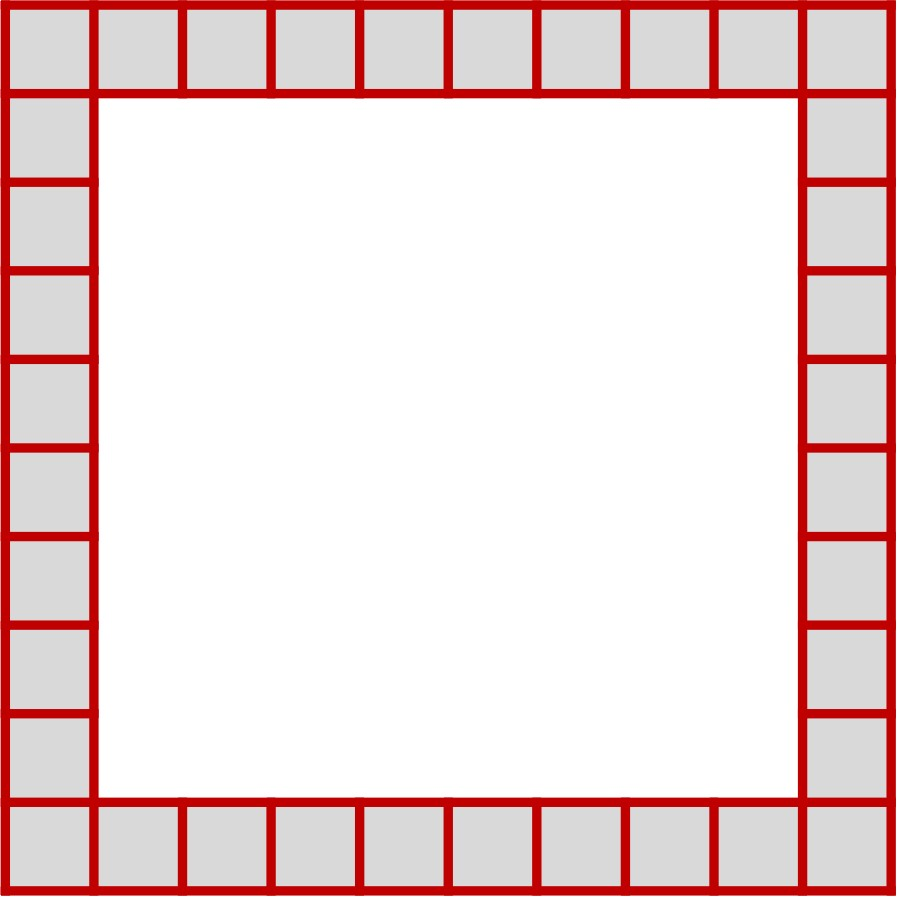
\includegraphics[width=0.4\linewidth]{10x10_Empty_Grid.jpg}<1->
        %\caption{\scriptsize{Basic model}}
        \label{fig:basic_model}
    \end{subfigure}%
    \begin{subfigure}{.5\textwidth}
        \centering
        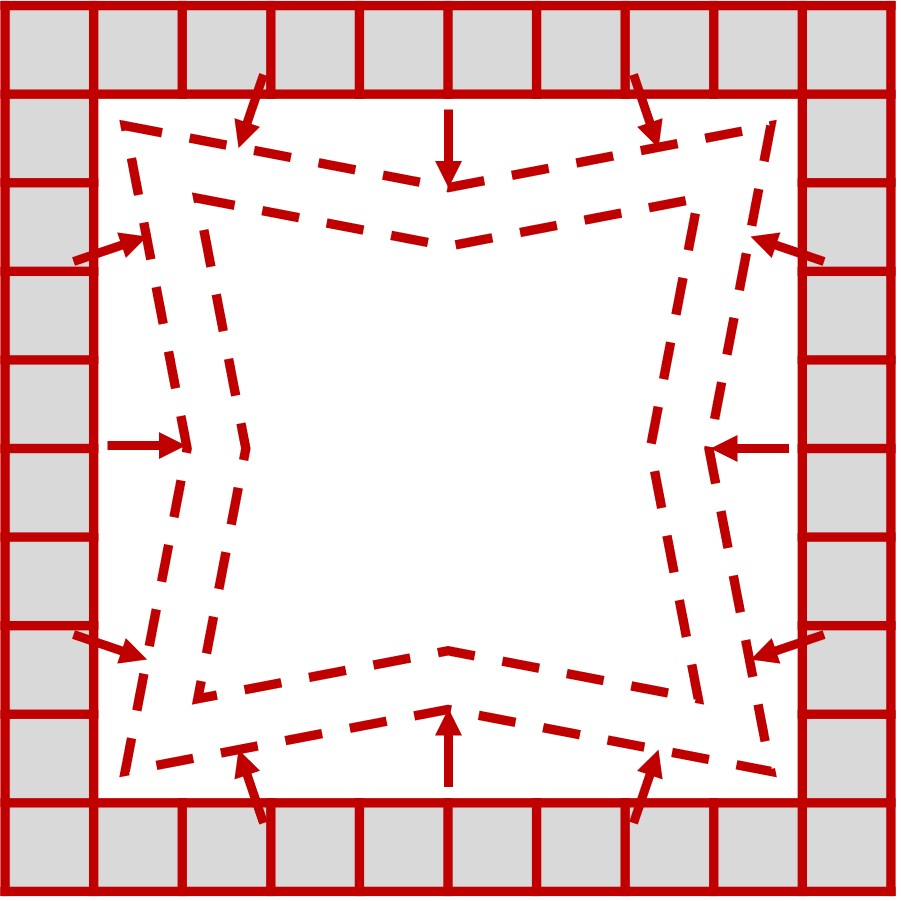
\includegraphics[width=0.4\linewidth]{10x10_Empty_Grid_Under_Pressure.jpg}<2->
        %\caption{\scriptsize{Basic model with pressure applied}}
        \label{fig:basic_model_pressure}
    \end{subfigure}
\end{frame}

%   Current Objectives------------------------------------------%

\begin{frame}
    \frametitle{Current Objectives (cont.)}
    \begin{itemize}
        \item<1-> Compare commercial software (NX 12, LSDyna, Marc Mentat)
    \end{itemize}
    \begin{center}
        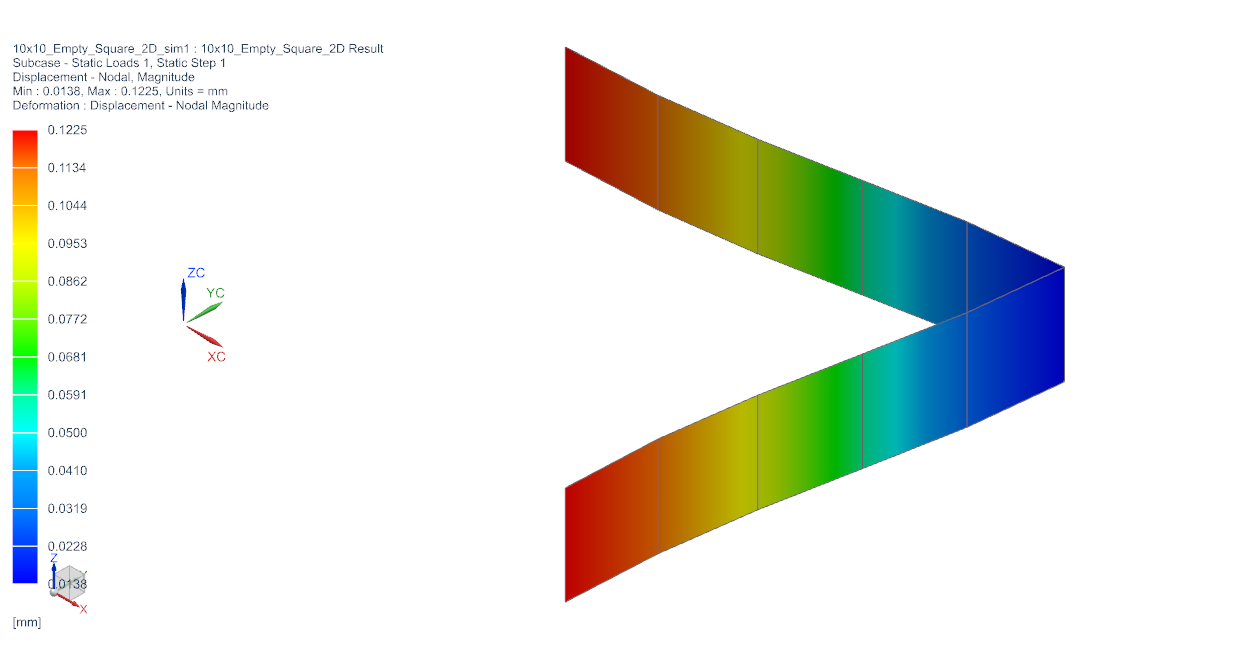
\includegraphics[width=0.35\linewidth]{10x10_Empty_Square_2D_Deformation.png}
    \end{center}
    \begin{itemize}
        \item<2-> Implementation with code from N Kim and open source software
    \end{itemize}
\end{frame}

%   Current Objectives------------------------------------------%

\begin{frame}
    \frametitle{Current Objectives (cont.)}
    \begin{itemize}
        \item<1-> Compare modeled behaviour to actual behaviour
        \changefontsizes{11pt}
        \begin{itemize}
            \item<2-> Produce square
            \item<2-> Place between two transparent plates
            \item<2-> Apply pressure
            \item<2-> Observe and compare
        \end{itemize}
        \item<3-> Determine which approach
        \changefontsizes{11pt}
        \begin{itemize}
            \item<4-> Commercial vs. open-source vs. own code
            \item<5-> All have pros and cons
        \end{itemize}
    \end{itemize}
\end{frame}

%   Further Objectives------------------------------------------%

\begin{frame}
    \frametitle{Further Objectives}
    \begin{itemize}
        \item<1-> Define unit cell behaviour
    \end{itemize}
    \begin{figure}
        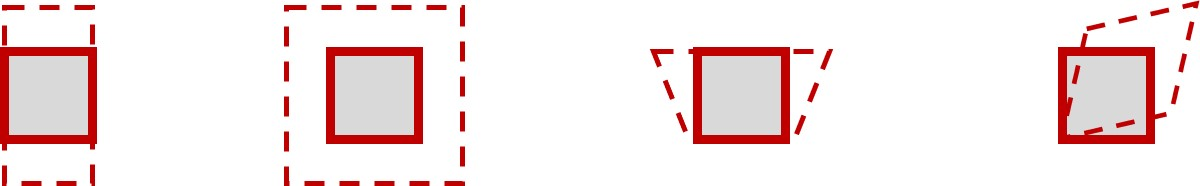
\includegraphics[height = 1cm]{Unit_Cell_Deformation.jpg}<1->
    \end{figure}
    \begin{itemize}
        \item<2-> Define recursive rules
        \item<3-> Set up genetic algorithm
        \item<4-> Combine all components
    \end{itemize}
\end{frame}

%   Questions---------------------------------------------------%

\begin{frame}
    \begin{center}
        \huge Questions?
    \end{center}
\end{frame}

\end{document}
